The position of each hexagon can be defined by the isometry from its canonical position; an isometry is given by the triple $\lr{\alpha, \beta, \delta}$ where $\alpha$ is a counter clockwise rotation about the center of the hexagon and $\lr{\beta,\delta}$ is a translation vector.% where $\beta$ is the translation of the obstacle hexagon in the $x$ axis and $\delta$ is the translation of the obstacle hexagon in the $y$ axis.
Canonical position would have each obstacle hexagon's position as $(0,0,0)$.
\begin{lem}\label{lem:aux-C}
Let P be a polygonal linkage obtained from the modified auxilary construction.  
In every realization of $P$, the obstacle polygons are close to canonical position such that 
\end{lem}
% The bottom most obstacle hexagon is glued to the side of the bottom frame hexagon.  
% The subsequent obstacle hexagons are rotated 
%Our goal is show that this quality cannot happen in the modified auxilary construction.  
Lemma \ref{lem:aux-C} serves as assurance that once a boolean formula of P3SAT is encoded into an arbitrary realization of the modified auxilary construction, the information of the boolean formula is preserved regardless of the positioning of the gadgets and components in the construction.
This quality shows that the information is stable and preserved in an arbitrary realization of the modified auxilary construction.
In Figure \ref{fig:tiltedObstaclesInFrame.pdf}, we have a column of obstacle hexagons veering off $\ell$.
This is an example of extreme angular rotation that should not occur over a vertical stack of hexagons.

% \begin{minipage}{\linewidth}
% \begin{center}
% \includegraphics[width=.3\columnwidth]{graphics/tiltedObstaclesInFrame.pdf}
% \captionof{figure}{This figure depicts a column of obstacle hexagons rotated such that the obstacle hexagons veer of the vertical line $\ell$.}\label{fig:tiltedObstaclesInFrame.pdf}
% \end{center}
% \end{minipage}
\begin{proof}
We need to show that the modified auxilary construction could not deform in such a way that any information the construction encodes is lost or modified and the functionality of the gadgets within the construction behave as stated in the description.

To help identify components of the construction for this proof, let's identify components in the canonical position:

\begin{minipage}{\linewidth}
\begin{center}
\includegraphics[width=.5\columnwidth]{graphics/smallHexagonalGridWithEll.pdf}
\captionof{figure}{This figure depicts a column of obstacle hexagons $O_1$, $\ldots$, $O_{10}$ along the vertical line $\ell$.}\label{fig:smallHexagonalGridWithEll.pdf}
\end{center}
\end{minipage}

Without loss of generality, we can identify a column of obstacle hexagons $O_i$ along a vertical line $\ell$ (See Figure \ref{fig:smallHexagonalGridWithEll.pdf}).
In this proof, unless otherwise specified, we assume that the argument refers to a column that starts and ends with an obstacle hexagon.  
In total there will be $u+1$ number of obstacle hexagons and $u$ corridors in a column. 

The length of $H(n,m)$ (and $\ell$ in Figure \ref{fig:corridorNonCanonical.pdf}) can be expressed as a sum of the heights of the corridors and obstacle polygons.
The width of a skinny rhombus in canonical position is $\frac{1}{100N}$.
The obstacle hexagon has height of $ (t+1) \cdot \sqrt{3}$, and the flag is of height $\sqrt{3}$.  
\begin{equation}\label{eqn:Hnm}
H(n,m) = (u+1) (t+1) \sqrt{3} + u \lr{\frac{1}{100N} + \sqrt{3}}
\end{equation}

\paragraph{Angular Rotation $\alpha$}
First we show that the angular rotation of the obstacle hexagons with respect to canonical position is small.  
We first look at the relative angular difference between two adjacent obstacle polygons
$$\left\vert \alpha_i - \alpha_{i+1} \right\vert.$$
Given an arbitrary instance of a modified auxilary construction, consider $O_i$, $O_{i+1}$, and the corridor between $O_i$ and $O_{i+1}$.
The skinny rhombus  has length $\sqrt{1 + \lr{100N}^{-2}}$.



\begin{minipage}{\linewidth}
\begin{center}
\includegraphics[width=.9\columnwidth]{graphics/corridorNonCanonical.pdf}
\captionof{figure}{The obstacle hexagon here is in noncanonical position, and showing the side lengths adjacent to $\alpha_i$.}\label{fig:corridorNonCanonical.pdf}
\end{center}
\end{minipage}

The cross section of an arbitrary corridor must have a height of at least $\sqrt{3}$ everywhere. 
%noncanonical corridor must be at least 
Otherwise, a flag would overlap with an obstacle hexagon; it would no longer remain a realization since the height of a flag is $\sqrt{3}$.
In Figure \ref{fig:corridorNonCanonical.pdf}, we illustrate an obstacle hexagon, its upper corridor with the flag that has the hinge to the skinny rhombus.  
The rhombus is hinged at the midpoint of the upper side of the corridor.
The length from a corridor's midpoint to one end of the corridor is $\frac{N}{2}$.
$\gamma_j$ is the angle between $s_j$ and the horizontal axis at the height of the flag ($j = 1,2,\ldots, u$).
The bound of $\gamma_j$ is:
\begin{equation}\label{eqn:gammaBound}
\begin{array}{rcl}
\gamma_j &\leq & \tan^{-1} \lr{
								\frac{
										\sqrt{1+ \lr{	\frac{1}{100N}	}^2}
								}{
										\frac{N}{2}
								}	
							}\\
&=& \tan^{-1} \lr{\frac{2\sqrt{1 + \frac{1}{(100N)^2}}}{N}}\\
&\leq& \frac{2\sqrt{1 + \frac{1}{(100N)^2}}}{N} - \frac{1}{3}\lr{\frac{2\sqrt{1 + \frac{1}{(100N)^2}}}{N}}^3\\
&=&\frac{\lr{6N^2 - 8 - \frac{8}{(100N)^2}}\cdot \sqrt{1 + \frac{1}{(100N)^2}} }{3N^3}\\
&\leq&\frac{\lr{6N^2 - 8 - \frac{8}{(100N)^2}}\cdot \frac{3}{2} }{3N^3}\\
&=&\frac{2\lr{3N^2 - 4 - \frac{4}{(100N)^2}}\cdot \frac{3}{2} }{3N^3}\\
&=&\frac{3N^2 - 4 - \frac{4}{(100N)^2}}{N^3}
\end{array} 
\end{equation}
Inequality \ref{eqn:gammaBound} uses the first two terms Maclaurin series of $\tan^{-1}$.
Thus the relative rotational difference between adjacent obstacle hexagons is
$$ \vert \alpha_i - \alpha_{i+1} \vert \leq \frac{3N^2 - 4 - \frac{4}{(100N)^2}}{N^3}$$
From this inequality, it is clear that as $N \rightarrow \infty$, $\gamma_j \rightarrow 0$; and so the relative difference between $\alpha_i$ and $\alpha_{i+1}$ goes to zero as well.

The cross section of the corridor must have a minimum height of $\sqrt{3}$ everywhere.
The height of an obstacle polygon in noncanonical position is $(t+1) \cdot \sec \alpha_i \cdot \sqrt{3}$.

\begin{minipage}{\linewidth}
\begin{center}
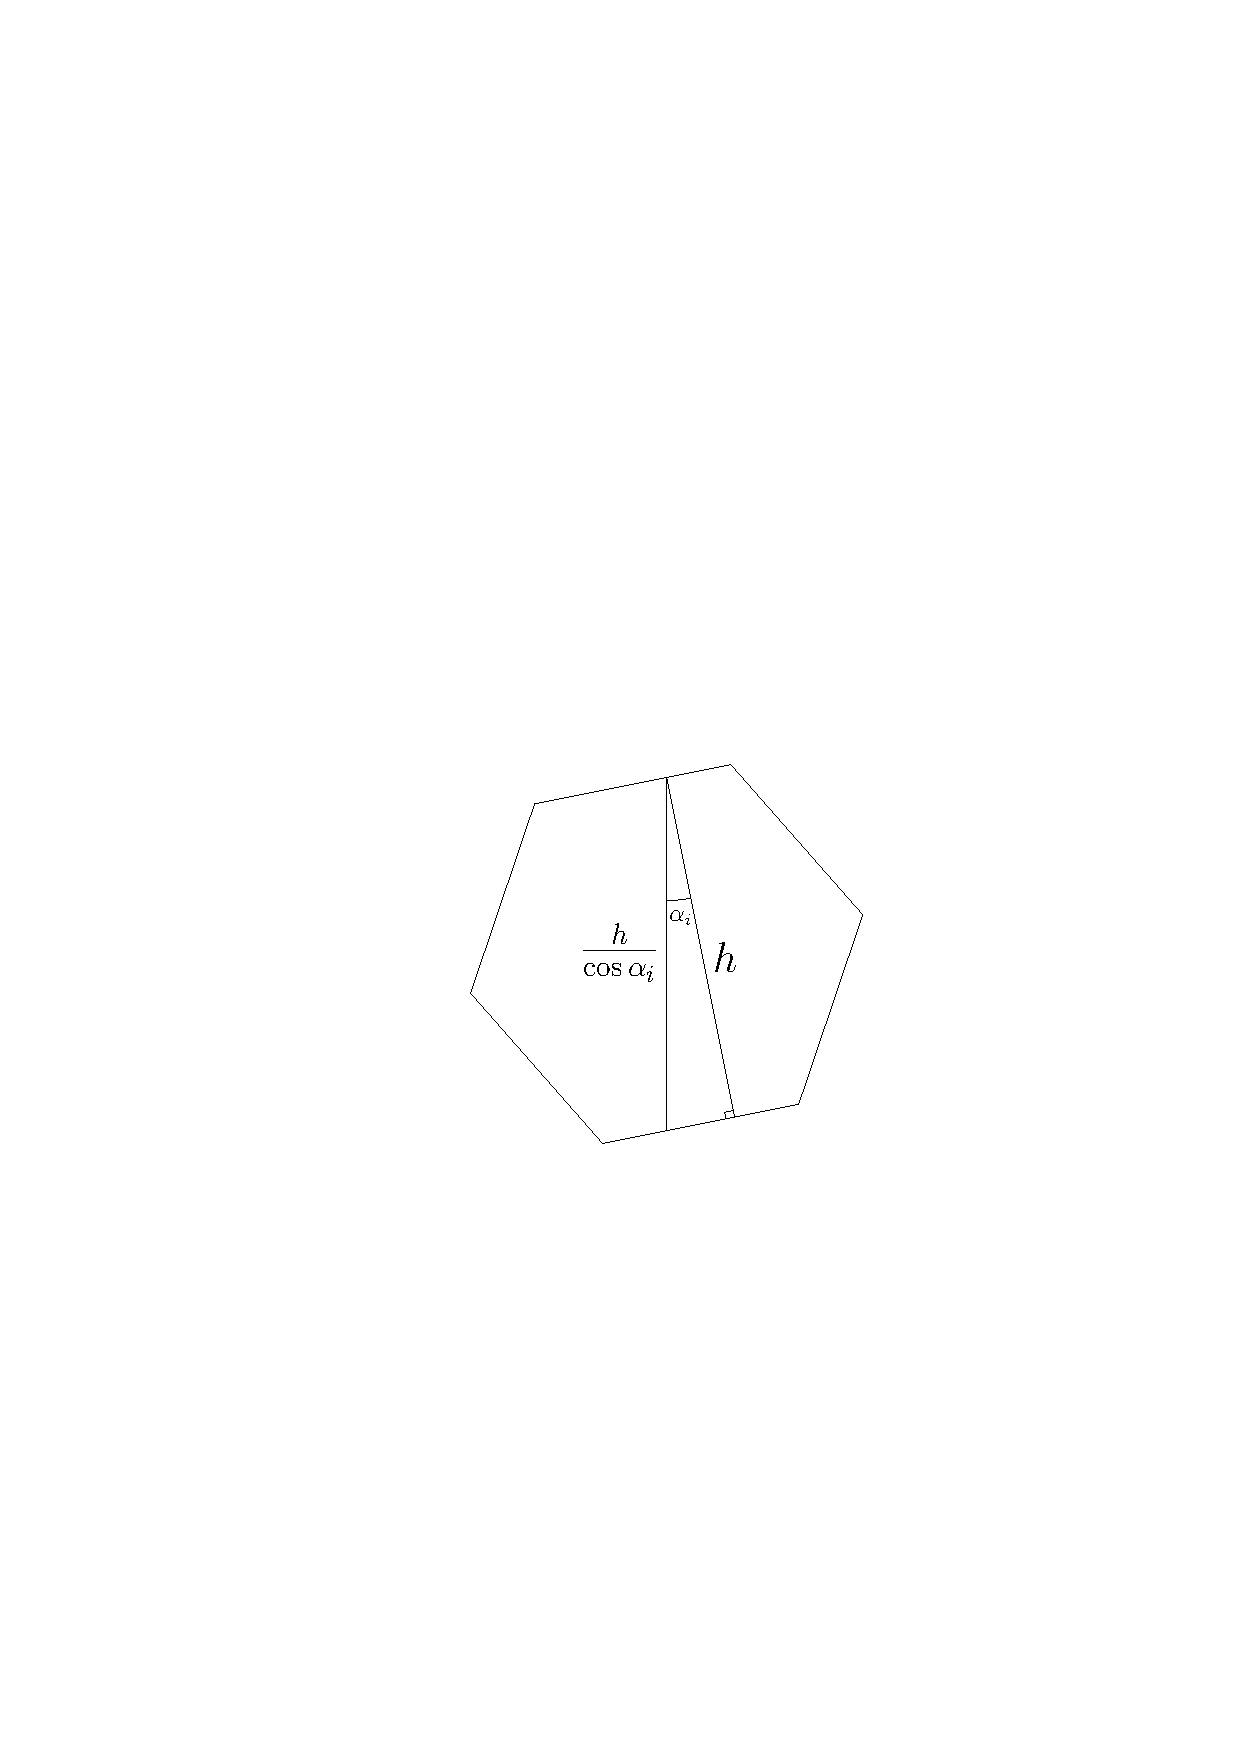
\includegraphics[width=.33\columnwidth]{graphics/hexagonNonCanonical2.pdf}
\captionof{figure}{
% The obstacle hexagon here is in non-canonical position, and showing the side lengths adjacent to $\alpha_i$.
This figure shows a right triangle with angle $\alpha_i$ and sides of length $h$ and $\frac{h}{\cos \alpha_i}$
}\label{fig:hexagonNonCanonical.pdf}
\end{center}
\end{minipage}

%The height of the cross section of an obstacle polygon and  
Figure \ref{fig:hexagonNonCanonical.pdf}, the height of the obstacle hexagon $h$ is $(t+1) \cdot \sqrt{3}$.  
When rotated by $\alpha_i$, $h$ becomes $h \sec \alpha_i$.
Using Equation \ref{eqn:Hnm} of $H(n,m)$, the length from the canonical position can also be represented as a sum of widths of corridors and cross sectional heights obstacle hexagons in arbtrary position:
\begin{eqnarray*}
H(n,m) = (u+1) (t+1) \sqrt{3} + u \lr{\frac{1}{100N} + \sqrt{3}}&=& \sum_{i=1}^{u} \sqrt{3} + \sum_{i=1}^{u+1} (t+1) \sqrt{3} \sec \alpha_i \\ 
&\leq& u \sqrt{3} + (t+1) \sqrt{3} \sum_{i = 1}^{u+1} \sec \alpha_i\\

\end{eqnarray*}
% \begin{eqnarray*}
% h_\text{max} = (u+1) (t+1) \sqrt{3} + u\lr{\sqrt{3}+ \frac{1}{100N}}&\geq& \sum_{i = 1}^{u+1} (t+1) \cdot \sec \alpha_i \cdot \sqrt{3} + m \sqrt{3}\\
% (m+1) (t+1) \sum_{i = 1}^{m+1} \lr{1 - \sec \alpha_i}&\geq& m \lr{\sqrt{3} - \lr{\sqrt{3}+ \frac{1}{100N}}}\\
% \sum_{i = 1}^{m+1} \lr{ \sec \alpha_i - 1} &\leq& \frac{m}{100 N \sqrt{3} (m+1)(t+1) }\\
% \sum_{i = 1}^{m+1} \lr{ \lr{1 + \frac{\alpha_i^2}{2}} - 1} &\leq&\frac{m}{100 N \sqrt{3} (m+1)\lr{\lr{2N^3 - 1}+1} }\\
% \sum_{i = 1}^{m+1} \frac{\alpha_i^2}{2} &\leq&\frac{m}{200 N^4 (m+1) \sqrt{3} } \\
% \sum_{i = 1}^{m+1} \alpha_i^2 &\leq& \frac{m}{100N^4 (m+1) \sqrt{3}}
% \end{eqnarray*}
% Focusing on the right hand side of the inequality above, we have the following result:
% \begin{eqnarray*}
% \frac{m}{100N^4 (m+1) \sqrt{3}} &<& \frac{m}{m+1}\\
% \frac{1}{100N^4 \sqrt{3}}&<& 1
% \end{eqnarray*}

As $N \rightarrow \infty$, $\frac{m}{100N^4 (m+1) \sqrt{3}} \rightarrow 0$ which implies $\sum_{i = 1}^{m+1} \alpha_i^2$ is bounded.  
The number of obstacle hexagons is determined by a polynomial $N(a,b)$ where $a$ is the number of variables in a corresponding Boolean formula and $b$ is the number of clauses in the Boolean formula.
Since $\alpha_i$ is bounded above, then there is a maximal rotation of each obstacle hexagon from canonical position.
Thus every realization of $P$, the obstacle polygons are close to canonical position.


\paragraph{Vertical Displacement $\delta$}
\paragraph{Horizontal Displacement $\alpha$}
\end{proof}